% TEXINPUTS=.:/home/hei2/Documents/LaTeX/myTexStyles:
% created for Journal of Heuristics 
% Time-stamp: "2011-07-18 14:17 hei2"
% if all fonts computer modern use -G1
% dvips -Ppdf -G0 <filename>
% http://www.springer.de/comp/lncs/authors.html

%!TEX TS-program = xelatex
%!TEX encoding = UTF-8 Unicode

%! xelatex joh.tex

\RequirePackage{fix-cm} 

\documentclass[twocolumn]{svjour3} 

\makeatletter
\def\cl@chapter{\@elt {theorem}}
\makeatother

\usepackage{mathptmx} % use Times fonts if available on your TeX system

\journalname{Journal of Scheduling}

\title{Discovering dispatching rules from data using imitation learning}
\subtitle{Case study for the job-shop problem}

\author{Helga Ingimundardottir \and Thomas Philip Runarsson}

\institute{H. Ingimundardottir \at
Dunhaga 5, IS-107 Reykjavik, Iceland \\
Tel.: +354-525-4704\\
Fax: +354-525-4632\\
\email{hei2@hi.is}\\
\and
T.P. Runarsson \at
Hjardarhagi 2-6, IS-107 Reykjavik, Iceland \\
Tel.: +354-525-4733\\
Fax: +354-525-4632\\
\email{tpr@hi.is}\\
}
\date{Received: \today / Accepted: date}
% The correct dates will be entered by the editor

\usepackage[english]{babel} 

% please place your own definitions here and don't use \def but
% \newcommand{}{}
\usepackage{url}

\usepackage{amssymb,bm,amsmath}
\newcommand{\vphi}{\bm{\phi}}
\newcommand{\vsigma}{\bm \sigma}
\newcommand{\vchi}{\bm \chi}
\newcommand{\R}{{\mathbb R}}

\newcommand{\inner}[2]{\big<{#1}\cdot{#2}\big>}
\newcommand{\abs}[1]{\lvert#1\rvert}
\newcommand{\norm}[1]{\lVert#1\rVert}
\newcommand{\argmax}{\mathop{\rm argmax}}
\newcommand{\nchoosek}[2]{\tiny \left(\begin{array}{c}#1\\#2\end{array}\right)}
\newcommand{\condset}[2]{\left\{#1\;\middle|\;#2\right\}}

% percentage relative deviation from optimality
\newcommand{\Namerho}{Deviation from optimality, $\rho$}
\newcommand{\namerho}{deviation from optimality, $\rho$}
\newcommand{\fullnamerho}{\namerho, defined by~\cref{eq:rho}}
\newcommand{\Problem}[2][ ]{$\mathcal{P}_{#2}^{#1}$}
\newcommand{\jrnd}[2]{\Problem[#1 \times #2]{j.rnd}}
\newcommand{\jrndJ}[2]{\Problem[#1 \times #2]{j.rnd,J_1}}
\newcommand{\jrndM}[2]{\Problem[#1 \times #2]{j.rnd,M_1}}
\newcommand{\jrndn}[2]{\Problem[#1 \times #2]{j.rndn}}
\newcommand{\frnd}[2]{\Problem[#1 \times #2]{f.rnd}}
\newcommand{\frndn}[2]{\Problem[#1 \times #2]{f.rndn}}
\newcommand{\fjc}[2]{\Problem[#1 \times #2]{f.jc}}
\newcommand{\fmc}[2]{\Problem[#1 \times #2]{f.mc}}
\newcommand{\fmxc}[2]{\Problem[#1 \times #2]{f.mxc}}
\newcommand{\dr}{dispatching rule}
\newcommand{\cdr}{composite priority \dr}
\newcommand{\sdr}{single priority \dr}
\newcommand{\Fsp}{Flow-shop}
\newcommand{\Jsp}{Job-shop}
\newcommand{\fsp}{flow-shop}
\newcommand{\jsp}{job-shop}
\newcommand{\FSP}{FSP}
\newcommand{\JSP}{JSP}
\newcommand{\Jrnd}{\JSP~random}
\newcommand{\JrndJ}{\JSP~random with job variation}
\newcommand{\JrndM}{\JSP~random with machine variation}
\newcommand{\Jrndn}{\JSP~random-narrow}
\newcommand{\Frnd}{\FSP~random}
\newcommand{\Frndn}{\FSP~random narrow}
\newcommand{\Fjc}{\FSP~job-correlated}
\newcommand{\Fmc}{\FSP~machine-correlated}
\newcommand{\Fmxc}{\FSP~mixed-correlated}

\newcounter{FeatCounter}
% job-related
\newcommand{\phiproc}{$\phi_1$}
\newcommand{\phistartTime}{$\phi_2$}
\newcommand{\phiendTime}{$\phi_3$}
\newcommand{\phiarrivalTime}{$\phi_4$}
\newcommand{\phitotalProc}{$\phi_5$}
\newcommand{\phiwait}{$\phi_6$}
\newcommand{\phiwrmJob}{$\phi_7$}
\newcommand{\phijobOps}{$\phi_8$}
\newcommand{\phiJobRelated}{\phiproc\!-\phijobOps}
% mac-related
\newcommand{\phimacFree}{$\phi_{9}$}
\newcommand{\phiwrmMac}{$\phi_{10}$}
\newcommand{\phimacOps}{$\phi_{11}$}
\newcommand{\phiMacRelated}{\phimacFree\!-\phimacOps}
% flow-related
\newcommand{\phislotsReduced}{$\phi_{12}$} 
\newcommand{\phislots}{$\phi_{13}$}
\newcommand{\phislotsTotal}{$\phi_{14}$} 
\newcommand{\phiFlowRelated}{\phislotsReduced\!-\phislotsTotal}
% schedule related
\newcommand{\phimakespan}{$\phi_{15}$}
\newcommand{\phiScheduleRelated}{\phimakespan}
% global
\newcommand{\phiSPT}{$\phi_{16}$}
\newcommand{\phiLPT}{$\phi_{17}$}
\newcommand{\phiLWR}{$\phi_{18}$}
\newcommand{\phiMWR}{$\phi_{19}$}
\newcommand{\phiRND}{$\phi_{20}$}
\newcommand{\phiSDRRelated}{\phiSPT\!-\phiMWR}
\newcommand{\phiGlobalRelated}{\phiMWR\!-\phiRND}
\newcommand{\phiLocalRelated}{\phiproc\!-\phimakespan}
\newcommand{\NrFeatLocal}{15}
\newcommand{\NrFeatGlobal}{5}
\newcommand{\NrFeatTotal}{20}

\hyphenation{heur-ist-ics}
\hyphenation{algo-rithm}

\usepackage{multirow}
\usepackage{rotating}
\newcommand{\rot}[1]{\begin{sideways}#1\end{sideways}}

\usepackage{paralist}

\usepackage{booktabs} % \toprule \midrule \bottomrule

\usepackage[colorinlistoftodos, textwidth=\marginparwidth]{todonotes}
\usepackage{comment}

\usepackage[capitalise,nameinlink]{cleveref} % must come last! % put your own shorthand declarations in this document

\begin{document}
\sloppy % fixes many bad boxes
\maketitle

\selectlanguage{english}

\begin{abstract}
  Over the years there have been many approaches to create \dr s for scheduling.
  Recent past efforts have focused on direct search methods (e.g. genetic 
  programming) or training on data (e.g. supervised learning).
  This paper will examine the latter and give a framework on how to do it 
  effectively. 
  Defining training data as  
  $\{\vec{x}_i(k),y_i(k)\}_{k=1}^K\in\mathcal{D}$ then
  \begin{enumerate*}
    \item features of partially constructed schedules $\vec{x}_i$ should 
    necessarily reflect the induced 
    data distribution $\mathcal{D}$ for when the rule is applied. This is achieved by updating the learned model in 
    an active imitation learning fashion
    \item $y_i$ is labelled optimally using a MIP solver
    \item data needs to be balanced, as the set is unbalanced w.r.t. 
    dispatching step $k$
  \end{enumerate*}
  
  When querying an optimal policy, there is an abundance of valuable 
  information that can be utilised for learning new models.
  For instance, it's possible to seek out when the scheduling process is most 
  susceptible to failure.
  Generally stepwise optimality (or classification accuracy) 
  will imply good end performance, here minimising the makespan. 
  However, as the impact of suboptimal moves is not fully understood, then the 
  measure needs to be adjusted for its intended trajectory.
 
  Using the guidelines set by the framework the design of custom \dr s, for 
  one's particular scheduling application, will be more effective. In the study 
  presented three different distributions of the \jsp\ will be considered.
  The machine learning approach considered is based on preference learning, 
  which learns what post decision state is preferable to another. However, 
  alternative learning methods may be applied to the training data generated.
  
  \keywords{Scheduling \and Composite \dr s \and Performance Analysis \and 
  Machine Learning \and Imitation Learning \and DAgger \and Preference Learning}
\end{abstract}

%\todo{story line:
%from heuristic design to supervised learning to data creating (data 
%distributed as it is used). Understanding the critical points in the 
%construction of solution ...}

\section{Introduction}\label{sec:introduction}

Hand crafting heuristics for scheduling is an ad-hoc approach to finding 
approximate solutions to the problems. The practice is time-consuming and its 
performance can even vary dramatically between different problem instances. The 
aim of this work is to increase our understanding of this process. In 
particular the learning of new problem specific priority \dr s (DR) will be 
addressed for a subclass of scheduling problems known as the \jsp\ scheduling 
problem (\JSP). 

A recent editorial of the state-of-the-art approaches \cite{Chen13} in advanced 
\dr s for large-scale manufacturing systems reminds us that:
\lq\lq ... most traditional \dr s are based on historical data. 
With the emergence of data mining and on-line analytic processing, dispatching 
rules can now take predictive information into account.\rq\rq~The importance of 
automated discovery of \dr s was also emphasised by \cite{Monch13}. 
Data for learning can also be generated using a known heuristic on a set of 
problem instances.
Such an approach is taken in \cite{Siggi05} for single-machine where
a decision tree is learned from the data to have similar logic to the guiding 
\dr. 
However, the learned method cannot outperform the original \dr\ for the data 
generation. 
This drawback is confronted in \cite{Malik08,Russell09,Siggi10} by using an 
optimal scheduler or policy, computed off-line, for data generation. The 
resulting \dr s, as decision trees, gave significantly better schedules than 
using popular heuristics in that field, and a lower worst-case factor from 
optimality. 
Although, using optimal policies for creating training data gives vital 
information on how to learn good scheduling rules we will show that this is 
not sufficient. Once these rules make a suboptimal dispatch then they are in 
uncharted territory and its effects are relatively unknown. 
This work will illustrate the sensitivity of learned \dr's performance on the 
way the training data is sampled.
For this purpose, \JSP\ is used as a case study to illustrate a methodology for 
generating meaningful training data, which can be successfully 
learned using preference-based imitation learning.

%Using improvement heuristics, \cite{Zhang95} studied space shuttle payload 
%processing by using reinforcement learning (RL), in particular, temporal 
%difference learning. 
%Starting with a relaxed problem, each job was scheduled as early as its 
%temporal partial order would permit, there by initially ignoring any resource 
%constraints on the machines, yielding the schedule's critical path. Then the 
%schedule would be repaired so the resource constraints were satisfied in the 
%minimum amount of iterations.

%Meta learning can be very fruitful in RL, as experiments from 
%\cite{Kalyanakrishnan11} discovered some key discriminants between 
%competing algorithms for their particular problem instances, which provided 
%them with a hybrid algorithm which combines the strengths of the algorithms.

% automation for selecting DRs #4 - GA
The competing alternative to learning dispatching rules from data would be to 
search the \dr\ space directly. The prevalent approach in this case would be 
using an evolutionary algorithm, such as genetic programming (GP).
The main drawback is that the rules from a GP framework can be quite complex, 
and difficult to interpret.
For instance \cite{Tay08} applied GP on a terminal set of job-attributes for 
flexible \jsp\ with promising results compared to the benchmarks DRs from the 
literature.
In fact, \cite{Hildebrandt2010} revisited the experiments from \cite{Tay08} 
that were reported to be successful for dynamic \jsp\ and tested it against 
some \sdr s and found out it only slightly outperformed one rule, 
and was beat by another. 
The reason behind this staggering change in performance, may be due to 
the choice of objective function or the underlying problem spaces that were 
used in training.
It's argued that randomly generated problem instances aren't a 
proper representative for real-world long-term \jsp\ applications, e.g., by the 
narrow choice of release times, yielding schedules that are overloading in the 
beginning phases.

A novel iterative \dr s that were evolved with GP for \JSP, \cite{Nguyen13} 
learned from completed schedules in order to iteratively improve new ones. 
At each dispatching step, the method can utilise the current feature space to 
\emph{correctify} some possible \emph{bad} dispatch made previously (sort of 
reverse lookahead). Their method computationally inexpensive, although the 
authors do stress that there is still remains room for improvement.
A simpler and more straightforward way to automate selection of \cdr s (CDR), 
\cite{InRu14}, translated \dr s into measurable attributes (or features) and 
optimise directly what their contribution should be via evolutionary search. 
%The framework is straight forward and easy to implement and showed promising 
%and robust results, as models were trained on a lower dimension, and validated 
%on higher dimension. 

The most predominant approach in hyper-heuristics is a framework of creating 
\emph{new} heuristics from a set of predefined heuristics via GA optimisation 
\cite{Burke10}. 
Adopting a two-stage hyper-heuristic approach to generate a set of 
machine-specific DRs for dynamic \jsp, \cite{Pickardt2013} used GP to evolve 
CDRs from basic attributes, along with evolutionary algorithm to assign 
a CDR to a specific machine. 
The problem space consists of \jsp s in semiconductor manufacturing, with 
additional shop constraints, as machines are grouped to similar work centres, 
which can have different set-up time, workload, etc. 
In fact, the GP emphasised on efficiently dispatching on the work centres with 
set-up requirements and batching capabilities, which are rules that are 
non-trivial to determine manually.

Using case based reasoning for timetable scheduling, training data in 
\cite{Burke06} is guided by the two best heuristics in the literature.
They point out that in order for their framework to be successful, problem 
features need to be sufficiently explanatory and training data needs to be 
selected carefully so they can suggest the appropriate solution for a specific 
range of new cases. 

% automation for selecting DRs #1 - Portfolio
With meta heuristics one can use existing DRs, and use for example 
portfolio-based algorithm selection \cite{Rice76,Gomes01,Xu07}, either based on 
a single instance or class of instances to determine which DR to choose from. 
% automation for selecting DRs #2 - ACO
Implementing ant colony optimisation to select the best DR 
from a selection of nine DRs for \JSP, experiments from \cite{Korytkowski13} 
showed that the choice of DR do affect the results and that for all performance 
measures considered. They showed that it was better to have a all the DRs to 
choose from rather than just a single DR at a time.

%Svo mætti koma ein málsgrein sem er samantekt á því sem aðrir hafa lært af 
%þessu öllu:
%1.) Features matter       2.) Training data matters
%3.) Problem specific      4.) Annað? Time depedendance
To summarise, when dealing with learning new \dr s there are several important 
factors to consider. First and foremost the meaningfulness of training data 
will influence the quality of the learned \dr. 
Since the training data consists of collection of features, the quality of 
training data is interchangeable to the predictability of features. 
Stressing the importance of consequential feature selection. 
Furthermore, the training data should be problem specific and as closely 
related to the final benchmark instances for relevant results. 
In addition to addressing these chosen aspects, the paper will show that during 
the scheduling process, it varies \emph{when} it's most fruitful to make the 
`right' decision, and depending on the distribution of problem instances those 
pivotal moments can vary greatly. 
Moreover, due to the nature of machine learning algorithm it's important to 
consider the actual end-performance when choosing a suitable model 
configuration, not just staring blindly at the classification accuracy as the 
relation between the two is elusive. 

The outline of the paper is the following, \cref{sec:problemdef} gives the 
mathematical formalities of the scheduling problem, and 
\cref{sec:DR} describes the main attributes for \jsp, 
and goes into how to create schedules with \dr s. 
\Cref{sec:learnOPT} sets up the framework for learning from optimal schedules. 
In particular, the probability of choosing optimal decisions and the effects of 
making a suboptimal decision. Furthermore, the optimality of common \sdr s is 
investigated.
With those guidelines, \cref{ch:expr:CDR} goes into detail how to create 
meaningful \cdr s using preference learning, focusing on how to 
compare operations and collect training data with the importance of good state 
sampling. 
\Cref{sec:il:active,sec:il:passive} explain the trajectories for 
sampling meaningful schedule state-spaces used in preference learning, either 
using passive or active imitation learning. 
Experimental results are jointly presented in \cref{sec:il:expr} with 
comparison for a single randomly generated problem space. Furthermore, some 
general adjustments for performance boost is also considered.
The paper finally concludes in \cref{sec:con} with discussion and conclusions.

\section{\Jsp~Scheduling}\label{sec:problemdef}
\JSP\ involves the scheduling of jobs on a set of 
machines. Each job consists of a number of operations which are then processed 
on the machines in a predetermined order. An optimal solution to the problem 
will depend on the specific objective. 
% For example, the optimal schedule may be the time needed to complete
% all jobs, i.e., the minimum makespan.

In this study we will consider the $n\times m$ \JSP, where $n$ jobs, 
$\mathcal{J}=\{J_j\}_{j=1}^n$, are scheduled on a finite set, 
$\mathcal{M}=\{M_a\}_{a=1}^m$, of $m$ machines. The index $j$ refers to a job 
$J_j\in\mathcal{J}$ while the index $a$ refers to a machine 
$M_a\in\mathcal{M}$. 
Each job requires a number of processing steps or operations, the pair 
$(j,a)$ refers to the operation, i.e., processing the task of job $J_j$ on 
machine $M_a$. 

Each job $J_j$ has an indivisible operation time (or cost) on machine $M_a$, 
$p_{ja}$, which is assumed to be integral and finite. 
Starting time of job $J_j$ on machine $M_a$ is denoted $x_s(j,a)$ and its 
end time is denoted $x_e(j,a)$ where:
\begin{equation}\quad x_e(j,a):=x_s(j,a)+p_{ja} \end{equation} 
Each job $J_j$ has a specified processing order through the machines. It is a 
permutation vector, $\vsigma_j$, of $\{1,\ldots,m\}$, representing a job $J_j$ 
can be processed on $M_{\vsigma_j(a)}$ only after it has been completely 
processed on $M_{\vsigma_j(a-1)}$, namely:
\begin{equation}\quad\label{eq:permutation}
x_s(j,\vsigma_j(a)) \geq x_e(j,\vsigma_j(a-1)) 
\end{equation}
for all $J_j\in\mathcal{J}$ and $a\in\{2,..,m\}$. 
Note, that each job can have its own distinctive flow pattern through the 
machines, which is independent of the other jobs. 
However, in the case that all jobs share the same \emph{fixed} permutation 
route, it is referred to as \fsp~(\FSP). 
A commonly used subclass of \FSP\ in the literature is permutation \fsp, which 
has the added constraint that the processing order of the jobs on the machines 
must be identical as well, i.e., no passing of jobs allowed \cite{Stafford88}.

The disjunctive condition that each machine can handle at most one job at a 
time is the following:
\begin{equation}\quad\label{eq:oneJobPerMac}
x_s(j,a) \geq x_e(j',a) \quad\textrm{or}\quad x_s(j',a) \geq x_e(j,a) 
\end{equation}
for all $J_j,J_{j'}\in\mathcal{J},\; J_j\neq J_{j'}$ and $M_a\in\mathcal{M}$. 

The objective function is to minimise the schedule's maximum completion times 
for all tasks, commonly referred to as the makespan, $C_{\max}$, which is 
defined as follows:
\begin{equation}\quad
C_{\max} := 
\max\left\{x_e(j,\vsigma_j(m))\;:\;J_j\in\mathcal{J}\right\}.\label{eq:makespan}
\end{equation} 
This family of scheduling problems is denoted by $J||C_{\max}$ 
\cite{Pinedo08}.
Additional constraints commonly considered are job release-dates and due-dates 
or sequence dependent set-up times, however, these will not be considered here. 

In order to find an optimal (or near optimal) solution for scheduling problems 
one could either use exact methods or heuristics methods. Exact methods 
guarantee an optimal solution. However, \jsp\ scheduling is strongly NP-hard 
\cite{Garey76:NPhard}. Any exact algorithm generally suffers from the curse of 
dimensionality, which impedes the application in finding the global optimum in 
a reasonable amount of time. 
Using state-of-the-art software for solving scheduling problems, such as 
LiSA %\footnote{LiSA is distributed under the GNU General Public License, and 
%is available at \url{http://www.math.ovgu.de/Lisa.html}.} 
(A Library of Scheduling Algorithms) \cite{LiSA}, which includes a specialised 
version of branch and bound that manages to find optimums for \jsp\ problems of 
up to $14\times14$ \cite{Ru12}. However, problems that are of greater size, 
become intractable. 
Heuristics are generally more time efficient but 
do not necessarily attain the global optimum. Therefore, \jsp\ has the 
reputation of being notoriously difficult to solve. 
As a result, it's been widely studied in deterministic scheduling theory and 
its class of problems has been tested on a plethora of different solution 
methodologies from various research fields \cite{Meeran12}, all from simple and 
straight forward \dr s to highly sophisticated frameworks.

\section{Priority Dispatching Rules} \label{sec:DR}

Priority \dr s determine, from a list of incomplete jobs, 
$\mathcal{L}$, which job should be dispatched next. This process, where an 
example of 
a temporal partial schedule of six-jobs scheduled on five-machines, is 
illustrated in \cref{fig:jssp:example}.
The numbers in the boxes represent the job identification $j$. 
The width of the box illustrates the processing times for a given job for a 
particular machine $M_a$ (on the vertical axis). 
The dashed boxes represent the resulting partial schedule for when a particular 
job is scheduled next. 
Moreover, the current $C_{\max}$ is denoted by a dotted vertical line. 
The object is to keep this value as small as possible once all operations are 
complete. As shown in the example there are $15$ operations already scheduled. 
The \textit{sequence} of dispatches used to create this partial schedule is:
\begin{equation}\quad
\vchi=\left(J_3,J_3,J_3,J_3,J_4,J_4,J_5,J_1,J_1,J_2,J_4,J_6,J_4,J_5,J_3\right)
\end{equation}
This refers to the sequential ordering of job dispatches to machines, i.e., 
$(j,a)$; 
the collective set of allocated jobs to machines is interpreted by its 
sequence which is referred to as a \emph{schedule}.
A \emph{scheduling policy} will pertain to the manner in which 
the sequence is determined from the available jobs to be scheduled. 
In our example, the available jobs are given by the job-list
$\mathcal{L}^{(k)}=\{J_1,J_2,J_4,J_5,J_6\}$ with the five potential jobs 
to be dispatched at step $k=16$ (note that $J_3$ is completed).

However, deciding which job to dispatch is not sufficient as one must also know 
where to place it. In order to build tight schedules it is sensible to place a 
job as soon as it becomes available and such that the machine idle time is 
minimal, i.e., schedules are non-delay. 
There may also be a number of different options for such a placement. 
In \cref{fig:jssp:example} one observes that $J_2$, to be scheduled on $M_3$, 
could be placed immediately in a slot between $J_3$ and $J_4$, or after $J_4$ 
on this machine. 
If $J_6$ had been placed earlier, a slot would have been created between it and 
$J_4$, thus creating a third alternative, namely scheduling $J_2$ after $J_6$. 
The time in which machine $M_a$ is idle between consecutive jobs $J_j$ and 
$J_{j'}$ is called idle time or slack:
\begin{equation}\quad 
s(a,j):=x_s(j,a)-x_e(j',a) \label{eq:slack}
\end{equation}
where $J_j$ is the immediate successor of $J_{j'}$ on $M_a$. 

Construction heuristics are designed in such a way that it limits the search 
space in a logical manner respecting not to exclude the optimum. Here, the 
construction heuristic, $\Upsilon$, is to schedule the dispatches as closely 
together as possible, i.e., minimise the schedule's idle time. 
More specifically, once an operation $(j,a)$ has been chosen from the job-list 
$\mathcal{L}$ by some dispatching rule, it can then be placed immediately after 
(but not prior) to $x_e(j,\vsigma_j(a-1))$ on machine $M_a$ due to constraint 
\cref{eq:permutation}. 
However, to guarantee that constraint \cref{eq:oneJobPerMac} is not violated, 
idle times $M_a$ are inspected as they create a slot which $J_j$ can 
occupy. Bearing in mind that $J_j$ release time is $x_e(j,\vsigma_j(a-1))$ one 
cannot implement \cref{eq:slack} directly, instead it has to be updated as 
follows:
\begin{equation}\quad
\tilde{s}(a,j'):= x_s(j'',a)-\max\{x_e(j',a),x_e(j,\vsigma_j(a-1))\} % 
%\textrm{ if } x_e(j,\vsigma_j(a-1)\geq x_e(j',a) 
\end{equation}
for all already dispatched jobs, $J_{j'},J_{j''}\in \mathcal{J}_a$ where 
$J_{j''}$ is $J_{j'}$ successor on $M_a$. Since preemption is not allowed, the 
only applicable slots are whose idle time can process the entire operation, 
namely:
\begin{equation}\quad
\tilde{S}_{ja} := \left\{J_{j'}\in \mathcal{J}_a \;:\; \tilde{s}(a,j')\geq p_{ja} 
\right\}\label{eq:slots}.
\end{equation} 
The placement rule applied will decide where to place the job and is intrinsic 
to the construction heuristic, which is chosen independently of the priority 
dispatching rule that is applied. 
Different placement rules could be considered for selecting a slot from 
\cref{eq:slots}, e.g., if the main concern were to utilise the slot space, then 
choosing the slot with the smallest idle time would yield a closer-fitted 
schedule and leave greater idle times undiminished for subsequent dispatches 
on $M_a$.
In our experiments, cases were discovered where such a placement could rule out 
the possibility of constructing optimal solutions.
However, this problem did not occur when jobs are simply placed as early as 
possible, which is beneficial for subsequent dispatches for $J_j$. 
For this reason, it will be the placement rule applied here.

\begin{figure}[t!]\centering
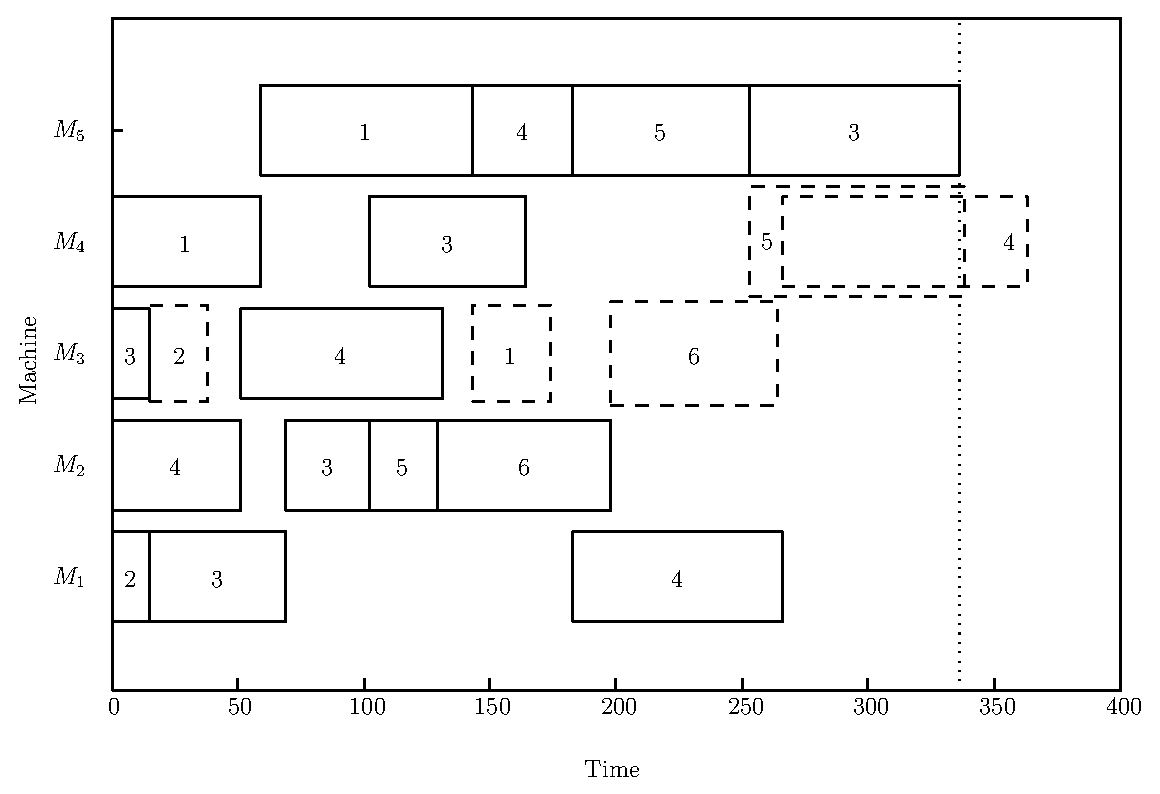
\includegraphics[width=\columnwidth]{figures/jssp_example}
\caption[Gantt chart of a partial \JSP\ schedule]{Gantt chart of a
partial \JSP\ schedule after 15 dispatches: Solid and dashed boxes
represent $\vchi$ and $\mathcal{L}^{(16)}$, respectively. Current
$C_{\max}$ denoted as dotted line.}
\label{fig:jssp:example}
\end{figure}

%Dispatching rules are of a construction heuristics, where one starts with an 
%empty schedule and adds sequentially on %one operation (or tasks) at a time. 

Priority \dr s will use attributes of operations, such as processing time, 
in order to determine the job with the highest priority. 
Consider again \cref{fig:jssp:example}, if the job with the shortest processing 
time (SPT) were to be scheduled next, then $J_2$ would be dispatched. 
Similarly, for the longest processing time (LPT) heuristic, $J_5$ would have 
the highest priority. 
Dispatching can also be based on attributes related to the partial schedule. 
Examples of these are dispatching the job with the most work remaining (MWR) or 
alternatively the least work remaining (LWR). A survey of more than $100$ of 
such rules are presented in \cite{Panwalkar77}. 
However, the reader is referred to an in-depth survey for simple or 
\emph{\sdr} (SDR) by \cite{Haupt89}. 
The SDRs assign an index to each job in the job-list and is generally only 
based on a few attributes and simple mathematical operations.

\begin{table}[t!] \centering
\caption[Attribute space $\mathcal{A}$ for \JSP]{Attribute space 
$\mathcal{A}$ for \JSP\ where job $J_j$ on machine $M_a$ given the 
resulting temporal schedule after operation $(j,a)$.
}
\label{tbl:jssp:feat}
{\setlength{\tabcolsep}{3pt} \centering
\renewcommand{\arraystretch}{1.5}
\begin{tabular}{clll} %p{0.45\textwidth}|p{0.4\textwidth}|}
	\toprule
	$\vphi$          & Feature description                       & Mathematical formulation                                                           & Shorthand    \\ 
	%\hline  \multicolumn{4}{c}{\textbf{Local features}}  \\
	\midrule
	\multicolumn{4}{c}{\textbf{job related}}\\
	\phiproc         & job processing time                       & $p_{ja}$                                                                           & proc         \\
	\phistartTime    & job start-time                            & $x_s(j,a)$                                                                         & startTime    \\
	\phiendTime      & job end-time                              & 
	$x_e(j,a)$                                                                    
	     &
	 endTime      \\
	\phiarrivalTime  & job arrival time                          & 
	$x_e(j,a-1)$                                                                  
	     &
	 arrival      \\ 
	\phitotalProc    & total processing time                     & $\sum_{a\in \mathcal{M}}p_{ja}$                                                    & totalProc    \\
	\phiwait         & time job had to wait                      & 
	$x_s(j,a)-x_e(j,a-1) 
	$                                                             & wait         
	\\   
	\phiwrmJob       & total work remaining for job              & $\sum_{a'\in\mathcal{M}\setminus \mathcal{M}_{j}}p_{ja'}$                          & wrmJob       \\
	\phijobOps       & number of assigned operations for job     & $|\mathcal{M}_j|$                                                                  & jobOps       \\ 
	\midrule
	\multicolumn{4}{c}{\textbf{machine related}}\\
	\phimacFree      & when machine is next free                 & $\max_{j'\in 
	\mathcal{J}_a} \{x_e(j',a)\}$                                         & 
	macFree      \\
	\phiwrmMac       & total work remaining for machine          & $\sum_{j'\in\mathcal{J}\setminus \mathcal{J}_{a}}p_{j'a} $                         & wrmMac       \\
	\phimacOps       & number of assigned operations for machine & $|\mathcal{J}_a|$                                                                  & macOps       \\
	\phislotsReduced & change in idle time by assignment         & $\Delta 
	s(a,j)$                                                                    & 
	reducedSlack \\
	\phislots        & total idle time for machine               & $\sum_{j'\in 
	\mathcal{J}_a}s(a,j')$                                                & 
	slack        \\
	\phislotsTotal   & total idle time for all machines          & $\sum_{a'\in 
	\mathcal{M}}\sum_{j'\in \mathcal{J}_{a'}}s(a',j')$                    & 
	totalSlack   \\
	\phimakespan     & current makespan                          & 
	$\max_{(j',a')\in \mathcal{J} \times 
	\mathcal{M}_{j'}}\{x_f(j',a')\}$              & makespan     \\
	\bottomrule
\end{tabular}

}
\end{table}

Designing priority \dr s requires recognising the important attributes of the 
partial schedules needed to create a reasonable scheduling rule. 
These attributes attempt to grasp key features of the schedule being 
constructed. Which attributes are most important will necessarily depend on the
objectives of the scheduling problem. 
Attributes used in this study applied for each possible operation encountered 
are given in \cref{tbl:jssp:feat}, where the set of machines already dispatched 
for $J_j$ is $\mathcal{M}_j\subset\mathcal{M}$, and similarly, $M_a$ has 
already had the jobs $\mathcal{J}_a\subset\mathcal{J}$ previously dispatched.
The attributes of particular interest were obtained by inspecting the 
aforementioned SDRs. Attributes \phiJobRelated\ and \phiMacRelated\ are 
job-related and machine-related, respectively.
In fact, \cite{Pickardt2013} note that in the current literature, there is a 
lack of global perspective in the attribute space, as omitting them won't 
address the possible negative impact an operation $(j,a)$ might have on other 
machines at a later time, it is for that reason we consider attributes such as 
\phiSlackRelated, that are slack related and are a means of indicating the 
current quality of the schedule.
All of the attributes, $\vphi$, vary throughout the scheduling process, 
w.r.t. operation belonging to the same time step $k$, with the exception of 
\phijobTotProcTime\ and \phimacTotProcTime\ which are static for a given 
problem instance but varying for each $J_j$ and $M_a$, respectively. 

Priority \dr s are attractive since they are relatively easy to 
implement, perform fast, and find reasonable schedules. In addition, they are 
relatively easy to interpret, which makes them desirable for the end-user.
However, they can also fail unpredictably. 
A careful combination of \dr s has been shown to perform significantly better 
\cite{Jayamohan04}. These are referred to as \emph{\cdr s} 
(CDR), where the priority ranking is an expression of several \dr s. 
CDRs deal with a greater number of more complicated functions (or features) and 
are constructed from the schedules attributes. In short, a CDR is a combination 
of several DRs. 
For instance let $\pi$ be a CDR comprised of $d$ DRs, then the index $I$ for 
$J_j\in\mathcal{L}^{(k)}$ using $\pi$ is:
\begin{equation}\quad I_j^{\pi} = \sum_{i=1}^d w_i \pi_i(\vchi^j) 
\label{eq:CDR}
\end{equation}
where $w_i>0$ and $\sum_{i=0}^d w_i = 1$ with $w_i$ giving the weight of the 
influence of $\pi_i$ (which could be a SDR or another CDR) to $\pi$. Note: 
each $\pi_i$ is a function of $J_j$'s attributes from the current sequence 
$\vchi$, where $\vchi^j$ implies that $J_j$ was the latest dispatch, i.e., the 
partial schedule given $\chi_k=J_j$.

At each step $k$, an operation is dispatched which has the highest 
priority. If there is a tie, some other priority measure is used. Generally 
the \dr s are static during the entire scheduling process. However, ties could 
also be broken randomly (RND). 

While investigating 11 SDRs for JSP, \cite{Lu13} a pool of 33 CDRs was created. 
This pool strongly outperformed the original CDRs by using multi-contextual 
functions based on either job waiting time or machine idle time (similar 
to \phiwait\ and \phimacSlack\ in \cref{tbl:jssp:feat}), i.e., the CDRs are a 
combination of either one or both of these key attributes and then the SDRs.
However, there are no combinations of the basic SDRs explored, only those two 
attributes. 
Similarly, using priority rules to combine 12 existing DRs from the literature, 
\cite{Yu13} had 48 CDR combinations which yielded 48 different models 
to implement and test. 
It is intuitive to get a boost in performance by introducing new CDRs, since 
where one DR might be failing, another could be excelling, so combining them 
together should yield a better CDR. However, these approaches introduce fairly 
ad-hoc solutions and there is no guarantee the optimal combination of 
\dr s are found.

The \cdr\ presented in \cref{eq:CDR} can be considered as a special case of a 
the following general linear value function:
\begin{equation}\quad\label{eq:jssp:linweights}
\pi(\vchi^j)=\sum_{i=1}^d w_i \phi_i(\vchi^j).
\end{equation}
when $\pi_i(\cdot)=\phi_i(\cdot)$, i.e., a composite function of the features 
from \cref{tbl:jssp:feat}. Finally, the job to be dispatched, $J_{j^*}$, 
corresponds to the one with the highest value, namely:
\begin{equation}\quad\label{eq:jstar}
J_{j^*}=\argmax_{J_j\in \mathcal{L}}\; \pi(\vchi^j)
\end{equation}
Similarly, \sdr s may be described by this linear model. For instance, let all 
$w_i=0$, but with following exceptions: $w_1=-1$ for SPT, $w_1=+1$ for LPT, 
$w_7=-1$ for LWR and $w_7=+1$ for MWR. Generally, the weights $\vec{w}$ are 
chosen by the designer or the 
rule apriori. A more attractive approach would be to learn these weights from 
problem examples directly. We will now investigate how this may be accomplished.

\section{Performance Analysis of Priority Dispatching Rules}\label{sec:learnOPT}

In order to create successful \dr s, a good starting point is to 
investigate the properties of optimal solutions and hopefully be able to learn 
how to mimic the construction of such solutions. For this, we follow optimal 
solutions, 
obtained by using a commercial software package \cite{gurobi} and inspect 
the probability of SDRs being optimal. This serves as an indicator of how hard 
it is to put our objective up as a machine learning problem. 
However, we must also take into consideration the end-goal, which is minimising 
\namerho, because of its relationship to stepwise, optimality is not fully 
understood.

In this \lcnamecref{sec:learnOPT} we will describe concerns that must be 
addressed when learning new priority \dr s. At the same time we will describe 
the experimental set-up used in our study. 
%The matters that must be addressed are as follows
%\begin{enumerate*}[itemjoin*={{, and finally }}]
%\item the problem instances used for learning and their optimal solutions
%\item the reconstruction of the optimal solution using a \dr
%\item the construction of the training set used for learning
%\item the machine learning algorithm applied
%\end{enumerate*}

\subsection{Problem Instances}\label{sec:data:sim}

The class of problem instances used in our studies is the \jsp\ scheduling 
problem described in \cref{sec:problemdef}. Each instance will have 
different processing times and machine ordering. Each instance will 
therefore create different challenges for a priority dispatching rule. 
Dispatching rules learned will be customised for the problems used for their 
training. For real world application using historical data would be most 
appropriate. The aim would be to learn a dispatching rule that works well on 
average for a given distribution of problem instances. 
To illustrate the performance difference of priority \dr s on different 
problem distributions within the same class of problems, 
consider the following three cases.
Problem instances for JSP are generated stochastically by fixing the number of 
jobs and machines to ten. A discrete processing time is sampled independently 
from a discrete uniform distribution from the interval $I=[u_1,u_2]$, i.e., 
$\vec{p}\sim \mathcal{U}(u_1,u_2)$. 
The machine order is a random permutation of all of the machines in the 
\jsp. Two different processing times distributions were explored, namely 
\jrnd{n}{m} where $I=[1,99]$ and \jrndn{n}{m} where $I=[45,55]$. These 
instances are referred to as random and random-narrow, respectively. In 
addition we consider the case where the machine order is fixed and the same for 
all jobs, i.e. $\sigma_j(a)=a$ for all $J_j\in\mathcal{J}$ and where 
$\vec{p}\sim\mathcal{U}(1,99)$. 
These jobs are denoted by \frnd{n}{m} and is analogous to \jrnd{n}{m}.
The problem spaces are summarised in \cref{tbl:data:sim}.

The goal is to minimise the makespan, $C_{\max}$. The optimum 
makespan is denoted $C_{\max}^{\pi_\star}$ (using the expert policy 
$\pi_\star$), and the makespan obtained from the 
scheduling policy $\pi$ under inspection by $C_{\max}^{\pi}$. Since the optimal 
makespan varies between problem instances the performance measure is the 
following:
\begin{equation}\quad\label{eq:rho}
\rho=\frac{C_{\max}^{\pi}-C_{\max}^{\pi_\star}}{C_{\max}^{\pi_\star}}\cdot
100\%
\end{equation}
which indicates the percentage relative deviation from optimality. 
Note: \cref{eq:rho} measures the discrepancy between predicted value and true 
outcome, and is commonly referred to as a loss function, which we would like to 
minimise for policy $\pi$.

\Cref{fig:boxplot:SDR} depicts the box-plot for \cref{eq:rho} when using the 
SDRs from \cref{sec:DR} for all of the problem spaces from \cref{tbl:data:sim}.
These box-plots show the difference in performance of the various SDRs. The 
rule MWR performs on average the best on the \jrnd{n}{m} and \jrndn{n}{m} 
problems instances, whereas for \frnd{n}{m} it is LWR that performs best. It is 
also interesting to observe that all but MWR perform statistically worse than a 
random job dispatching on the \jrnd{n}{m} and \jrndn{n}{m} problems instances.

\begin{table}\centering
\caption[Problem space distributions used in experimental studies.]{Problem 
space distributions used in experimental studies. Note, problem instances 
are synthetic and each problem space is i.i.d. 
}\label{tbl:data:sim}
{\renewcommand{\arraystretch}{1.5}
	\begin{tabular}{clcccl}\toprule 
		type & name & size ($n\times m$) & $N_{\text{train}}$ & 
		$N_{\text{test}}$ & note
		\\ \midrule
		\multirow{2}{*}{{JSP}}
		%&\jrnd{8}{8} &$8\times8$& -- & 500 & random \\
		  & \jrnd{10}{10}  & $10\times10$ & 300 & 200 & random        \\
		%&\jrnd{12}{12} &$12\times12$& -- & 500 & random \\
		%&\jrndn{8}{8} &$8\times8$& -- & 500 & random-narrow \\ 
		  & \jrndn{10}{10} & $10\times10$ & 300 & 200 & random-narrow \\ 
		%&\jrndn{12}{12} &$12\times12$& -- & 500 & random-narrow \\ 
		\midrule
		\multirow{1}{*}{{FSP}}
		%&\frnd{8}{8} &$8\times8$& --&500& random \\ 
		  & \frnd{10}{10}  & $10\times10$ & 300 & 200 & random        \\ 
		%&\frnd{12}{12} &$12\times12$& --&500& random \\ 
		\bottomrule
	\end{tabular}
}
\end{table} 

\begin{figure}
\centering
\includegraphics[width=\columnwidth]{figures/{boxplotRho_SDR_10x10}.pdf}
\caption{Box-plot for deviation from optimality, $\rho$, (\%) for SDRs}
\label{fig:boxplot:SDR}
\end{figure}

\subsection{Reconstructing optimal solutions}\label{sec:opt:sdr}

When building a complete schedule, $K=n\cdot m$ dispatches must be made 
sequentially. A job is placed at the earliest available time slot for its next 
machine, whilst still fulfilling that each machine can handle at most one job 
at each time, and jobs need to have finished their previous machines according 
to their machine order. Unfinished jobs from the job-list $\mathcal{L}$ are 
dispatched one at a time according to a deterministic 
scheduling policy (or heuristic). This process is given as a pseudo-code is 
given in \cref{pseudo:constructJSP}. 
After each dispatch\footnote{Dispatch and time step are used interchangeably.} 
the schedule's current features are updated based on 
the half-finished schedule, $\vchi$. 
For each possible post-decision state the temporal features are collected (cf. 
\cref{pseudo:constructJSP:phi}) forming the feature set, $\Phi$, based on all 
$N_{\text{train}}$ problem instances available, namely:
\begin{equation}\quad \label{eq:Phi}
\Phi := \bigcup_{\{\vec{x}_i\}_{i=1}^{N_{\text{train}}}} 
\left\{\vphi^j \;:\; J_j\in\mathcal{L}^{(k)}\right\}_{k=1}^K
\subset\mathcal{F}
\end{equation}
where the feature space $\mathcal{F}$ is described in \cref{tbl:jssp:feat}, and 
are based on job- and machine-attributes which are widespread in practice.

\begin{algorithm}[t]
    \caption{Pseudo code for constructing a \JSP\ sequence using a 
    deterministic scheduling policy rule, $\pi$, 
    for a fixed construction heuristic, $\Upsilon$.} 
    \label{pseudo:constructJSP}
    \begin{algorithmic}[1]
        \Procedure{Schedule\JSP}{$\pi,\Upsilon$}
        \State $\vchi \gets \emptyset$  
        \Comment{initial current dispatching sequence}
        \For{k}{1}{K=n\cdot m} 
        \Comment{at each dispatch iteration}
        \ForAll{$J_j\in \mathcal{L}^{(k)}\subset \mathcal{J}$} 
        \Comment{inspect job-list}
        \State $\vphi^j \gets \vphi\circ\Upsilon\left(\vchi^j\right)$ 
        \label{pseudo:constructJSP:phi}
        \Comment{temporal features for post-descision state $J_j$}
        \State $I_j^{\pi} \gets \pi\left(\vphi^j\right)$ 
        \Comment{priority for $J_j$}
        \EndFor
        \State $j^* \gets \argmax_{j\in \mathcal{L}^{(k)}}\{I_j^{\pi}\}$ 
        \Comment{choose highest priority}
        \State $\chi_k \gets J_{j^*}$ 
        \Comment{dispatch $j^*$}
        \EndFor
        \State \Return $C_{\max}^{\pi} \gets \Upsilon(\vchi)$ 
        \Comment{makespan and final schedule}
        \EndProcedure
    \end{algorithmic}
\end{algorithm}

%\subsection{Labelling schedules w.r.t. optimal decisions}
It is easy to see that the sequence of task assignments is by no means unique. 
Inspecting a partial schedule further along in the dispatching process such as 
in \cref{fig:jssp:example}, then let's say $J_1$ would be dispatched next, and 
in the next iteration $J_2$. Now this sequence would yield the same schedule as 
if $J_2$ would have been dispatched first and then $J_1$ in the next iteration, 
i.e., these are jobs with non-conflicting machines. 
In this particular scenario, one cannot infer that choosing $J_1$ is better 
and $J_2$ is worse (or vice versa) since they can both yield the same solution.
Furthermore, 
there may be multiple optimal solutions to the same 
problem instance. Hence not only is the sequence representation `flawed' in the 
sense that slight permutations on the sequence are in fact equivalent w.r.t. 
the end-result, but very varying permutations on the dispatching sequence 
(although given the same partial initial sequence) can result in very different 
complete schedules yet can still achieve the same makespan. 
%Care must be taken in this case that neither resulting features are labelled 
%as undesirable. Only the resulting features from a dispatch resulting in a 
%suboptimal solution should be labelled undesirable.

The redundancy in building optimal solutions using dispatching rules means that 
many different dispatches may yield an optimal solution to the problem instance.
Let's formalise the probability of optimality (or stepwise 
classification accuracy) for a given policy $\pi$, as:
\begin{equation}\quad \label{eq:tracc:opt}
\xi^\star_{\pi} := \mathbb{E}_{\pi_\star}\left\{\pi_{\star} = \pi \right\}
\end{equation}
that is to say the mean likelihood of our policy $\pi$ being equivalent to the 
expert policy $\pi_\star$.
The probability that a job chosen by a SDR yields an optimal makespan on a 
step-by-step basis, i.e., $\xi^\star_{\langle \text{SDR} \rangle}$, is depicted 
in \cref{fig:opt:SDR:xistar}. These probabilities
vary quite a bit between the different problem instances distributions studied. 
From \cref{fig:opt:SDR:xistar} it is observed that $\xi^\star_{\text{MWR}}$ has 
a higher probability than random guessing, in choosing a dispatch which may 
result in an optimal schedule. This is especially true towards the end of the 
schedule building process. 
Similarly, $\xi^\star_{\text{LWR}}$ chooses dispatches 
resulting in optimal schedules with a higher probability. This would appear to 
be support the idea that the higher the probability of dispatching jobs that 
may lead to an optimal schedule, the better the SDRs performance, as 
illustrated by \cref{fig:boxplot:SDR}. However, there is a counter example, 
$\xi^\star_{\text{SPT}}$ has a higher probability than random dispatching of 
selecting a jobs that may lead to an optimal solution. Nevertheless, the random 
dispatching performs better than SPT on problem instances \jrnd{10}{10} and 
\jrndn{10}{10}. 

\begin{figure}[t]
\centering
\includegraphics[width=\columnwidth]{figures/{trdat_prob_moveIsOptimal_10x10_SDR_xistar}.pdf}
\caption{Probability of SDR being optimal, 
$\xi^\star_{\langle\text{SDR}\rangle}$}
\label{fig:opt:SDR:xistar}
\end{figure}

Looking at \cref{fig:opt:SDR:xistar}, then \jrnd{10}{10} has a relatively high 
probability ($70\%$ and above) of choosing an optimal job at random. 
However, it is imperative to keep making optimal decisions, because the 
consequences of making suboptimal dispatches are unknown. 
To demonstrate this \cref{fig:case} depicts mean worst and best case scenario 
of the resulting \namerho, once off the optimal track, defined as follows:
\begin{subequations}\label{eq:bwc:opt}
\begin{eqnarray} 
\quad \zeta_{\min}^{\star}(k) &:=& \mathbb{E}_{\pi_\star}\left\{
\min_{J_j\in\mathcal{L}^{(k)}}(\rho) \;:\;
\forall C_{\max}^{\vchi^j} \gneq C_{\max}^{\pi_\star} \right\} \\
\quad \zeta_{\max}^{\star}(k) &:=& \mathbb{E}_{\pi_\star}\left\{
\max_{J_j\in\mathcal{L}^{(k)}}(\rho) \;:\;
\forall C_{\max}^{\vchi^j} \gneq C_{\max}^{\pi_\star} \right\}
\end{eqnarray}
\end{subequations}
Note, that this is given that there is only made \emph{one} non-optimal dispatch. 
Generally, there will be more, and then the compound effects of making 
suboptimal decisions cumulate. 

It is interesting to observe that for \jrnd{10}{10} and \jrndn{10}{10} making 
suboptimal decisions later impacts on the resulting makespan more than doing a 
mistake early. 
The opposite seems to be the case for \frnd{10}{10}. 
In this case it is imperative to make good decisions right from the start. This 
is due to the major structural differences between \JSP\ and \FSP, namely the 
latter having a homogeneous machine ordering, constricting the solution 
immensely. 

\begin{figure}[t]
\centering
\includegraphics[width=\columnwidth]{figures/{stepwise_10x10_OPT_casescenario}.pdf}
\caption{Mean deviation from optimality, $\rho$, (\%), for best and worst 
case scenario of making \emph{one} suboptimal dispatch (i.e. 
$\zeta^{\star}_{\min}$ and $\zeta^{\star}_{\max}$), depicted as lower and 
upper bound, respectively, for \jrnd{10}{10}, \jrndn{10}{10} and 
\frnd{10}{10}. Moreover, mean suboptimal move is given as a dashed line.}
\label{fig:case}
\end{figure}

\subsection{Blended \dr s}\label{sec:opt:bdr}
A naive approach to create a simple blended \dr~(BDR) would be to 
switch between SDRs at a predetermined time.
Observing again \cref{fig:opt:SDR:xistar}, a presumably good BDR for 
\jrnd{10}{10} would be to start with $\xi^\star_{\text{SPT}}$ and then switch 
over to $\xi^\star_{\text{MWR}}$ at around time step $k=40$, where the SDRs 
change places in outperforming one another. 
A box-plot for $\rho$ for the BDR compared with MWR and SPT is depicted in 
\cref{fig:boxplot:BDR} and its main statistics are reported in 
\cref{tbl:BDR:stats}. 
This simple swap between SDRs does outperform the SPT heuristic, yet 
doesn't manage to gain the performance edge of MWR. Using SPT downgrades the 
performance of MWR.
A reason for this lack of performance of our proposed BDR is perhaps that by 
starting out with SPT in the beginning, it sets up the schedules in such a way 
that it's quite greedy and only takes into consideration jobs with shortest 
immediate processing times. Now, even though it is possible to find optimal 
schedules from this scenario, as \cref{fig:opt:SDR:xistar} shows, the inherent 
structure that's already taking place might make it hard to come across by 
simple methods. Therefore it's by no means guaranteed that by simply swapping 
over to MWR will handle that situation which applying SPT has already created. 
\Cref{fig:boxplot:BDR} does however show, that by applying MWR instead of SPT 
in the latter stages, does help the schedule to be more compact w.r.t. SPT. 
However, the fact remains that the schedules have diverged too far from what 
MWR would have been able to achieve on its own. 

\begin{figure}[t]
\centering
\includegraphics[width=\columnwidth]{figures/j_rnd/{boxplotRho_BDR_10x10}.pdf}
\caption{Box-plot for deviation from optimality, $\rho$, (\%) for BDR where 
SPT is applied for the first 10\%, 15\%, 20\%, 30\% or 40\% of the 
dispatches, followed by MWR}
\label{fig:boxplot:BDR}
\end{figure}
\begin{table}[b]
\caption{Main statistics for \jrnd{10}{10} \namerho, using BDR that changes 
from SDR at a fixed time step $k$.}\label{tbl:BDR:stats} 
\centering
\begin{tabular}{ccrlrrrrrr}
  \toprule
  SDR \#1 & SDR \#2 & $k$ & Set & Min. & 1st Qu. & Median & Mean & 
    3rd Qu. & Max. \\ \midrule
  SPT & -- & $K$ & train & 20.38 & 41.15 & 50.70 & 51.31 & 59.18 & 94.20 \\ 
  SPT & -- & $K$ & test & 22.75 & 41.39 & 49.53 & 50.52 & 58.60 & 93.03 \\ 
  MWR & -- & $K$ & train & \textbf{4.42} & \textbf{17.84} & \textbf{21.74} & 
  22.13 & 26.00 & 47.78 \\ 
  MWR & -- & $K$ & test & \textbf{3.37} & \textbf{17.07} & 21.39 & 21.65 & 
  25.98 & \textbf{41.80} \\ 
  SPT & MWR & 10 & train & 5.54 & 17.98 & 21.75 & \textbf{21.99} & 
  \textbf{25.43} & \textbf{44.02} \\ 
  SPT & MWR & 10 & test & 5.87 & 17.29 & \textbf{20.78} & \textbf{21.28} & 
  \textbf{24.67} & 44.47 \\ 
  SPT & MWR & 15 & train & 4.76 & 18.24 & 22.04 & 22.49 & 26.65 & 49.86 \\ 
  SPT & MWR & 15 & test & 7.42 & 17.60 & 21.38 & 21.83 & 25.45 & 45.98 \\ 
  SPT & MWR & 40 & train & 13.04 & 23.42 & 28.12 & 28.94 & 33.67 & 54.98 \\ 
  SPT & MWR & 40 & test & 8.55 & 24.20 & 28.16 & 28.98 & 33.20 & 57.21 \\ 
  \bottomrule
\end{tabular}
\end{table}

In \cref{fig:opt:SDR:xistar} we inspected the stepwise optimality, given that 
we were on the optimal trajectory. Since we're bound to make mistakes at some 
points, it's interesting to see how that stepwise optimality evolves for its 
intended trajectory, thereby updating \cref{eq:tracc:opt} to:
\begin{equation}\quad \label{eq:tracc:track}
\xi_{\pi} := \mathbb{E}_{\pi}\left\{\pi_{\star} = \pi \right\}
\end{equation}
\Cref{fig:opt:SDR:xi} shows the log likelihood for $\xi_{\langle 
\text{SDR} \rangle}$ using \jrnd{10}{10}.
There we can see that even though $\xi_{\text{SPT}}$ is generally more 
likely to find optimal dispatches in the initial steps, then shortly after 
$k=15$, $\xi_{\text{MWR}}$ becomes a 
contender again. This could explain why our BDR switch at $k=40$ from 
\cref{fig:boxplot:BDR} was unsuccessful. However, changing to MWR at $k\leq20$
is not statistically significant from MWR (boost in mean $\rho$ 
is at most -0.5\%). 
But as pointed out for \cref{fig:case}, it's not so fatal to 
make bad moves in the very first dispatches for \jrnd{10}{10}, hence little 
gain with improved classification accuracy in that region. 
However, after $k>20$ then the BDR starts diverging from MWR. 

\begin{figure}[t]
\centering
\includegraphics[width=\columnwidth]{figures/j_rnd/{trdat_prob_moveIsOptimal_10x10_SDR_xi}.pdf}
\caption{Log likelihood of SDR being optimal for \jrnd{10}{10}, when 
following its corresponding SDR trajectory, i.e.,  
$\log\left(\xi_{\langle\text{SDR}\rangle}\right)$}
\label{fig:opt:SDR:xi}
\end{figure}

\section{Preference Learning}\label{ch:expr:CDR}
\Cref{sec:opt:bdr} demonstrated there is definitely something to be gained by
trying out different combinations of DRs, it's just non-trivial how to go about 
it, and motivates how it's best to learn such interaction, which 
will be addressed in this \lcnamecref{ch:expr:CDR}.

Learning models considered in this study are based on ordinal regression in 
which the learning task is formulated as learning preferences. In the case of 
scheduling, learning which operations are preferred to others. Ordinal 
regression has been previously presented in \cite{Ru06:PPSN} and in 
\cite{InRu11a} for \JSP, and given here for completeness. 

The optimum makespan is known for each problem instance. At each time step $k$, 
a number of feature pairs are created. 
Let $\vphi^{o}\in\mathcal{F}$ denote the post-decision state when dispatching 
$J_o\in\mathcal{O}^{(k)}$ corresponds to an optimal schedule being built. 
All post-decisions states corresponding to suboptimal dispatches, 
$J_s\in\mathcal{S}^{(k)}$, are denoted by $\vphi^{s}\in\mathcal{F}$.
Note, \mbox{$\mathcal{O}^{(k)}\cup\mathcal{S}^{(k)}=\mathcal{L}^{(k)}$}, and 
\mbox{$\mathcal{O}^{(k)}\cap\mathcal{S}^{(k)}=\emptyset$}.

The approach taken here is to verify analytically, at each time step, by fixing 
the current temporal schedule as an initial state, whether it is possible to 
\emph{somehow} yield an optimal schedule by manipulating the remainder of the 
sequence. This also takes care of the scenario that having dispatched a job 
resulting in a different temporal makespan would have resulted in the same 
final makespan if another optimal dispatching sequence would have been chosen. 
That is to say the training data generation takes into consideration when there 
are multiple optimal solutions\footnote{
There can be several optimal solutions available for each problem instance. 
However, it is deemed sufficient to inspect only one optimal trajectory per 
problem instance as there are $N_{\text{train}}=300$ independent instances 
which gives the training data variety.} 
to the same problem instance. 

Let's label features from \cref{eq:Phi} that were considered optimal, 
\mbox{$\vpsi^{o}=\vphi^{o}-\vphi^{s}$}, and suboptimal, 
\mbox{$\vpsi^{s}=\vphi^{s}-\vphi^{o}$} by $y_o=+1$ and $y_s=-1$ respectively. 
Then, the preference learning problem is specified by a set of preference pairs:
\begin{eqnarray}
\quad \Psi &=& 
\left\{\left(\vpsi^o,+1\right),\left(\vpsi^s,-1\right)
\;:\;
\forall \left(J_o,J_s\right) \in \mathcal{O}^{(k)} \times 
\mathcal{S}^{(k)}\right\}_{k=1}^{K} \nonumber
\\ &\subset& \Phi\times Y \label{eq:prefset}
\end{eqnarray}
where $\Phi\subset \mathbb{R}^d$ is the training set of $d=\NrFeatLocal$ 
features (cf. \cref{tbl:jssp:feat}), $Y=\{+1,-1\}$ is the outcome space from 
job pairs $J_o\in\mathcal{O}^{(k)}$ and $J_s\in\mathcal{S}^{(k)}$, for all 
dispatch steps $k$.

To summarise, each job is compared against another job of the job-list, 
$\mathcal{L}^{(k)}$, and if the makespan differs (i.e 
$C_{\max}^{\pi_\star(\vchi^s)} \gneq C_{\max}^{\pi_\star(\vchi^o)}$) an 
optimal/suboptimal pair is created. 
However, if the makespans are identical the pair is omitted since they give the 
same optimal makespan. 
This way, only features from a dispatch resulting in a suboptimal solution is 
labelled undesirable.

Now let's consider the model space $\mathcal{H} = \{\pi(\cdot) : X \mapsto Y\}$ 
of mappings from solutions to ranks. Each such 
function $\pi$ induces an ordering on the solutions by the following rule:
\begin{equation}\quad\label{eq:linear}
\vchi^i \succ \vchi^j \quad \Leftrightarrow \quad \pi(\vchi^i) > 
\pi(\vchi^j)
\end{equation}
where the symbol $\succ$ denotes ``is preferred to.'' The function used to 
induce the preference is defined by a linear function in the feature space:
\begin{equation}\quad 
\pi(\vchi^j)=\sum_{i=1}^d w_i\phi_i(\vchi^j)=\inner{\vec{w}}{\vphi(\vchi^j)}.
\end{equation}

Logistic regression learns the optimal parameters $\vec{w}^*\in\mathbb{R}^d$. 
For this study, L2-regularised logistic regression from the \textsc{liblinear} 
package \cite{liblinear} without bias is used to learn the preference set 
$\Psi$, defined by \cref{eq:prefset}.
%For each job on the job-list, $J_j\in\mathcal{L}$, the post-decision state is 
%$\vphi^j:=\vphi(\vchi^j)$. 
Hence the job chosen to be dispatched, $J_{j^*}$, is the one corresponding to 
the highest preference estimate, i.e., \cref{eq:jstar} where $\pi(\cdot)$ is 
the classification model obtained by the preference set.

Preliminary experiments for creating step-by-step model was done in 
\cite{InRu11a} resulting in local linear model for each dispatch; a total of 
$K$ linear models for solving $n\times m$ JSP. 
However, the experiments there showed that by fixing the weights to its mean 
value throughout the dispatching sequence results remained satisfactory.
A more sophisticated way would be to create a \emph{new} linear model, where 
the preference set, $\Psi$, is the union of the preference pairs across the 
$K$ dispatches, such as described in \cref{eq:prefset}. 
This would amount to a substantial preference set, and for $\Psi$ to be 
computationally feasible to learn, $\Psi$ has to be reduced. For this several 
ranking strategies were explored in \cite{InRu15a}, the results there showed 
that it's sufficient to use partial subsequent rankings, namely, combinations 
of $r_i$ and $r_{i+1}$ for $i\in\{1,\ldots,n'\}$, are added to the preference 
set, where $r_1>r_2>\ldots>r_{n'}$ ($n'\leq n$) are the rankings of the 
job-list, in such a manner that in the cases that there are more than one 
operation with the same ranking, only one from that rank is needed to be 
compared to the subsequent rank. 
Moreover, for this study, which deals with $10\times 10$ problem instances 
instead of $6\times5$, the partial subsequent ranking becomes necessary, as 
full ranking is computationally infeasible due to its size. 
Defining the size of the preference set as $l=\abs{\Psi}$, then if $l$ is too 
large re-sampling to size $l_{\max}$ may be needed to be done in order for the 
ordinal regression to be computationally feasible. 

%\subsection{Collecting training data}
The training data from \cite{InRu11a} was created from optimal solutions of 
randomly generated problem instances, i.e., traditional \emph{passive} 
imitation learning (IL). 
As \JSP\ is a sequential decision making process, errors are bound to emerge. 
Due to compound effect of making suboptimal dispatches, the model leads the 
schedule astray from learned state-spaces, resulting in the new input being 
foreign to the learned model. 
Alternatively, training data could be generated using suboptimal solution 
trajectories as well, as was done in \cite{InRu15a}, where the training data 
also incorporated following the trajectories obtained by applying successful 
SDRs from the literature. 
The reasoning behind it was that they would be beneficial for learning, 
as they might help the model to escape from local minima once off the coveted 
optimal path. 
Simply aggregating training data obtained by following the trajectories of 
well-known SDRs yielded better models with lower \namerho. 

Inspired by the work of \cite{RossB10,RossGB11}, the methodology of generating 
training data will now be such that it will iteratively improve upon the model, 
such that the state-spaces learned will be representative of the state-spaces 
the eventual model would likely encounter, known as DAgger for \emph{active} 
imitation learning.
Thereby, eliminating the ad-hoc nature of choosing trajectories to learn, by 
rather letting the model lead its own way in a self-perpetuating manner until 
it converges.

Furthermore, in order to boost training accuracy, two strategies were explored 
\begin{enumerate}[after={{}}, leftmargin=*,
label={\textbf{Boost.\arabic*}}, ref={{Boost.\arabic*}}]
\item \label{expr:boost:varylmax} increasing number of preferences used 
in training (i.e. varying \mbox{$l_{\max} \leq \abs{\Psi}$}),
\item \label{expr:boost:newdata} introducing more problem instances (denoted 
EXT in experimental setting).
\end{enumerate}
Note, the following experimental studies will address 
\ref{expr:boost:newdata}, whereas preliminary experiments for 
\ref{expr:boost:varylmax} showed no statistical significance in boost of 
performance. Hence, the default set-up will be $l_{\max}=5 \cdot 10^5$ which is 
roughly the amount of features encountered from one pass of sampling a 
\mbox{$K$-stepped} trajectory using a fixed policy $\pi$ for the default 
$N_{\text{train}}=300$. 

Another way to adjust training accuracy is to give different weight to various 
time steps. To address this problem, two different stepwise sampling biases (or 
data balancing techniques) will be considered
\begin{enumerate}[after={{}}, leftmargin=*,
label={\textbf{Bias.\arabic*}}, ref={{Bias.\arabic*}}]
\item \label{bias:equal} \textbf{(equal)} where each time step has equal 
probability, this was used in \cite{InRu14,InRu15a} and serves as a baseline.
\item \label{bias:adjdbl2nd} \textbf{(adjdbl2nd)} where each time step is 
adjusted to the number of preference pairs for that particular step (i.e. 
each step now has equal probability irrespective of quantity of encountered 
features). This is done with re-sampling.
In addition, there is superimposed twice as much likelihood of 
choosing pairs from the latter half of the dispatching process. Then the 
final sampled data set is divided as follows:
$\abs{\{\Psi(k)\}_{k=0}^{\frac{K}{2}-1}} \approx \frac{1}{3}l_{\max}$ and 
$\abs{\{\Psi(k)\}_{k=\frac{K}{2}}^{K-1}} \approx \frac{2}{3}l_{\max}$.
\end{enumerate}

\noindent Remark: as the following \lcnamecref{sec:il:passive}s require 
repeated collection of training data, and since its labelling is a very 
time intensive task the remainder of the paper will solely be focusing 
on \jrnd{10}{10}.

\section{Passive Imitation Learning}\label{sec:il:passive}
Using the terms from game-theory used in \cite{CesaBianchi06}, % chapter 2: 
then our problem is a basic version of the sequential prediction problem where 
the predictor (or forecaster), $\pi$, observes each element of a sequence 
$\vchi$ of jobs, where at each time step $k \in \{1,...,K\}$, before the 
$k$-th job of the sequence is revealed, the predictor guesses its value 
$\chi_k$ on the basis of the previous $k-1$ observations. 

\subsection{Prediction with Expert Advice}\label{sec:expertPolicy}
Let's assume we know the expert policy $\pi^\star$, which we can query what 
is the optimal choice of $\chi_k={j^*}$ at any given time step $k$. 
Now we can use \cref{eq:jstar} to back-propagate the relationship between 
post-decision states and $\hat{\pi}$ with preference learning via our collected 
feature set, denoted $\Phi^\text{OPT}$, i.e., we collect the features set 
corresponding following optimal tasks $J_{j^*}$ from $\pi^\star$ in 
\cref{pseudo:constructJSP}.
This baseline sampling trajectory originally introduced in \cite{InRu11a} for 
adding features to the feature set is a pure strategy where at each dispatch an 
optimal task is dispatched.

By querying the expert policy, $\pi_\star$, the ranking of the job-list, 
$\mathcal{L}$, is determined such that:
\begin{equation}\quad
r_1 \succ r_2 \succ \cdots \succ r_{n'} \quad (n' \leq n)
\end{equation}
implies $r_1$ is preferable to $r_2$, and $r_2$ is preferable to $r_3$, etc. 
In our study, we know $r \propto C_{\max}^{\pi_\star}$, hence the optimal 
job-list is the following:
\begin{equation}\quad
\mathcal{O}=\left\{r_i \;:\; r_i \propto \min_{J_j \in \mathcal{L}} 
C_{\max}^{\pi_\star(\vchi^j)}\right\}
\end{equation}
found by solving the current partial schedule to optimality using a MIP solver.

When $\abs{\mathcal{O}^{(k)}}>1$, there can be several trajectories worth 
exploring. However, only one is chosen at random. This is deemed sufficient as 
the number of problem instances, $N_{\text{train}}$, is relatively large.

\subsection{Follow the Perturbed Leader}\label{sec:perturbedLeader}
By allowing a predictor to randomise it's possible to achieve improved 
performance \cite{CesaBianchi06,Hannan57}. This is the inspiration for our next 
strategy called Follow the Perturbed Leader, denoted OPT$\epsilon$. 
Its pseudo code is given in \cref{pseudo:perturbedLeader} and describes how the 
expert policy (i.e. optimal trajectory) from \cref{sec:expertPolicy} is subtly
``perturbed'' with $\epsilon=10\%$ likelihood, by choosing a job corresponding 
to the second best $C_{\max}$ instead of a optimal one with some small 
probability. 

\begin{algorithm}[t]
    \caption[Perturbed leader]{Pseudo code for choosing job 
    $J_{j^*}$ following a perturbed leader.}
    \label{pseudo:perturbedLeader}
    \begin{algorithmic}[1]
        \Require Ranking $r_1 \succ r_2 \succ \cdots > r_{n'} ~ (n' \leq n)$ of 
        the job-list, $\mathcal{L}$ \Comment{query $\pi_\star$}
        \Procedure{PerturbedLeader}{$\mathcal{L},\pi_\star$}
        \State $\epsilon \gets 0.1$ \Comment{likelihood factor}
        \State $p \gets \mathcal{U}(0,1)\in [0,1]$
        \Comment{uniform probability}
        \State $\mathcal{O} \gets \condset{j\in\mathcal{L}}{r_j=r_1}$ 
        \Comment{optimal job-list}
        \State $\mathcal{S} \gets \condset{j\in\mathcal{L}}{r_j>r_1}$
        \Comment{sub-optimal job-list}
        \If {$p < \epsilon \algorithmicand n'>1$} 
        \State \Return $j^* \in \condset{j\in\mathcal{S}}{r_j=r_2}$ 
        \Comment{any second best job}
        \Else 
        \State \Return $j^* \in\mathcal{O}$ \Comment{any optimal job}
        \EndIf
        \EndProcedure
    \end{algorithmic}
\end{algorithm}

\subsection{Experimental study}\label{sec:pil:expr}

\begin{figure}
\includegraphics[width=\columnwidth]{figures/{j_rnd}/{boxplot_passive_10x10}.pdf}
\caption{Box plot for \jrnd{10}{10} \namerho, using either expert policy and 
following perturbed leader.}\label{fig:passive:boxplot} 
\end{figure}

Results for \cref{sec:expertPolicy,sec:perturbedLeader} using \jrnd{10}{10} 
box-plot of \namerho, is given in \cref{fig:passive:boxplot} and main 
statistics are reported in \cref{tbl:IL:stats}. 
To address \ref{expr:boost:newdata}, the extended training set was simply 
obtained by iterating over more examples, namely $N^{\text{OPT}}_{\text{train, 
EXT}}=1000$. However, we see that the increased number of varied features 
dissuades the preference models to achieving a good performance w.r.t. $\rho$. 
It's preferable to use the default $N^{\text{OPT}}_{\text{train}}=300$ and 
allowing slight perturbations of the optimal trajectory, as done for 
$\Phi^{\text{OPT}\epsilon}$. Unfortunately, all this overhead has not managed 
to surpass MWR in performance, except for $\Phi^{\text{OPT}\epsilon}$ using 
\ref{bias:adjdbl2nd} with a $\Delta\rho\approx-4.24\%$ boost in mean 
performance. Otherwise, for \ref{bias:equal}, there is a loss of 
$\Delta\rho\approx+6.23\%$ in mean performance. 
This is likely due to the fact that if equal probability is used for stepwise 
sampling, then there are hardly any emphasis given to the final dispatches as 
there a relatively few (compared to previous steps) preference pairs belonging 
to those final stages.
Revisiting \cref{fig:case}, then the band for 
$\{\zeta^{\star}_{\min},\zeta^{\star}_{\max}\}$ is quite tight, as the problem 
is immensely constricted and few operations to choose from. However, the 
empirical evidence from using \ref{bias:adjdbl2nd} shows that it is 
imperative to make right decisions at the very end.

From \cite{InRu11a} we know that expert policy is a promising starting point.
However, that was for $6\times5$ dimensionality (i.e. $K=30$), which is a much 
simpler problem space. Notice that in \cref{fig:opt:SDR:xi} there was 
virtually no chance for $\xi_\pi(k)$ of choosing a job resulting in optimal 
makespan after step $k=28$.
Since \jsp\ is a sequential prediction problem, all future observations are 
dependent on previous operations. 
Therefore, learning sampled states that correspond only to optimal or 
near-optimal schedules isn't of much use when the preference model has 
diverged too far. We know from \cref{sec:opt:bdr}, that good classification 
accuracy based on $\xi^\star_\pi$ doesn't necessarily mean a low mean \namerho.
This is due to the learner's predictions affects future input observations 
during its execution, which violates the crucial i.i.d. assumptions of the 
learning approach, and ignoring this interaction leads to poor performance.
In fact, \cite{RossB10} proves that assuming the preference model has a 
training error of $\epsilon$, then the total compound error (for all $K$ 
dispatches) the classifier induces itself grows quadratically, $\bigOh{\epsilon 
K^2}$, for the entire schedule, rather than having linear loss, 
$\bigOh{\epsilon K}$, if it were i.i.d.

\section{Active Imitation Learning}\label{sec:il:active}

To amend performance from $\Phi^{\text{OPT}}$-based models, suboptimal 
state-spaces were explored in \cite{InRu15a} by inspecting the features from 
successful SDRs, $\Phi^{\langle\text{SDR}\rangle}$, by passively observing a 
full execution of following the task chosen by the corresponding SDR. 
This required some trial-and-error as the experiments showed that features 
obtained by SDR trajectories were not equally useful for learning.

To automate this process, inspiration from \emph{active} imitation learning 
presented in \cite{RossGB11} is sought, called \emph{Dataset Aggregation} 
(DAgger) method, which addresses a no-regret algorithm in an on-line learning 
setting. 
The novel meta-algorithm for IL learns a deterministic policy guaranteed to 
perform well under its induced distribution of states. 
The method is closely related to Follow-the-leader (cf. 
\cref{sec:il:passive}), however, with a more sophisticated leverage to the 
expert policy. 
In short, it entails the model $\pi_i$ that queries an expert policy (same as 
in \cref{sec:expertPolicy}), $\pi_\star$, it's trying to mimic, 
but also ensuring the learned model updates itself in an iterative fashion, 
until it converges. 
The benefit of this approach is that the states that are likely to occur in 
practice are also investigated and as such used to dissuade the model from 
making poor choices. In fact, the method queries the expert about the desired 
action at individual post-decision states which are both based on \emph{past} 
queries, and the learner's interaction with the \emph{current} environment.

DAgger has been proven successful on a variety of benchmarks 
\cite{RossGB11,Ross13}, such as the video games Super Tux Kart and Super 
Mario Bros., handwriting recognition and autonomous navigation for large 
unmanned aerial vehicles. In all cases greatly improving traditional supervised 
imitation learning approaches.

\subsection{DAgger}
The policy of imitation learning at iteration $i>0$ is a mixed strategy given 
as follows:
\begin{equation}\quad\label{eq:il}
\pi_i = \beta_i\pi_\star + (1-\beta_i)\hat{\pi}_{i-1}
% i: ith iteration of imitation learning
% pi_star is expert policy (i.e. optimal)
% pi_i^hat: is pref model from prev. iteration
\end{equation}
where $\pi_\star$ is the expert policy and $\hat{\pi}_{i-1}$ is the learned 
model from the previous iteration. 
Note, for the initial iteration, $i=0$, a pure strategy of $\pi_\star$ is 
followed. Hence, $\hat{\pi}_0$ corresponds to the preference model from 
\cref{sec:expertPolicy} (i.e. $\Phi^{\text{IL}0}=\Phi^{\text{OPT}}$). 

\Cref{eq:il} shows that $\beta_i$ controls the probability distribution of 
querying the expert policy $\pi_\star$ instead of the previous imitation model, 
$\hat{\pi}_{i-1}$. 
The only requirement for $\{\beta_i\}_i^\infty$ according to \cite{RossGB11} is 
that $\limit{\frac{1}{T}\sum_{i=0}^T\beta_i}{T\to\infty}{0}$ to guarantee 
finding a policy $\hat{\pi}_i$ that achieves $\epsilon$ surrogate loss under 
its own state distribution limit.

\Cref{pseudo:activeIL} explains the pseudo code for how to collect 
partial training set, $\Phi^{\text{IL}i}$ for $i$-th iteration of active 
imitation learning.
Subsequently, the resulting preference model, $\hat{\pi}_i$, learns on the 
aggregated datasets from all previous iterations, namely:
\begin{equation}\quad\label{eq:DAgger}
\Phi^{\text{DA}i}=\bigcup_{i'=0}^{i}\Phi^{\text{IL}i'}
\end{equation}
and its update procedure is detailed in \cref{pseudo:DAgger}.

% pi_i = beta_i*pi_star + (1-beta_i)*pi_i^hat
% i: ith iteration of imitation learning
% pi_star is expert policy (i.e. optimal)
% pi_i^hat: is pref model from prev. iteration

\begin{algorithm}[t]
    \caption[Active imitation learning]{Pseudo code for choosing job 
    $J_{j^*}$ using imitation learning (dependent on iteration $i$) to collect 
    training set $\Phi^{\text{IL}i}$; either by following optimal trajectory, 
    $\pi_\star$, or preference model 
    %based on aggregated preference sets, $\bigcup_{i'=0}^{i-1}S^{\text{IL}i'}$,
    from previous iterations, $\hat{\pi}_{i-1}$.}
    \label{pseudo:activeIL}
    \begin{algorithmic}[1]
        \Require $i\geq0$ 
        \Require Ranking $r_1 \succ r_2 \succ \cdots > r_{n'} ~ (n' \leq n)$ of 
                the job-list, $\mathcal{L}$ \Comment{query $\pi_\star$}
        \Procedure{ActiveIL}{$i,\hat{\pi}_{i-1},\pi_\star$}
        \State $p \gets \mathcal{U}(0,1)\in [0,1]$
        \Comment{uniform probability}
        \If{$i>0$} ~ (unsupervised)
        \State $\beta_i \gets 0$ 
        \Comment{always apply imitiation}
        \Else ~ (fixed supervision)  \State $\beta_i \gets 1$ 
        \Comment{always follow expert policy (i.e. optimal)}
        \EndIf
        \If {$p > \beta_i$} 
        \State \Return $j^* \gets \argmax_{j\in 
        \mathcal{L}}\{I_j^{\hat{\pi}_{i-1}}\}$
        \Comment{best job based on $\hat{\pi}_{i-1}$, 
        cf.~\cref{pseudo:constructJSP}}
        \Else 
        \State $\mathcal{O} \gets \condset{j\in\mathcal{L}}{r_j=r_1}$ 
        \Comment{optimal job-list}
        \State \Return $j^* \in\mathcal{O}$ \Comment{any optimal job}
        \EndIf
        \EndProcedure
    \end{algorithmic}
\end{algorithm}
\begin{algorithm}[t]
    \caption{DAgger: Dataset Aggregation for \JSP}
    \label{pseudo:DAgger}
    \begin{algorithmic}[1]
        \Require $T\geq1$
        \Procedure{DAgger}{$\pi_\star,\Phi^\text{OPT},T$}
        \State $\Phi^{\text{IL}0} \gets \Phi^{\text{OPT}}$ \Comment{initialize 
        dataset}
        \State $\hat{\pi}_0 \gets$ \Call{Train}{$\Phi^{\text{IL}0}$}
        \Comment{initial model, equivalent to \cref{sec:expertPolicy}}
        \For{i}{1}{T} \Comment{at each imitation learning iteration}
        \State Let $\pi_i = \beta_i\pi_\star + (1-\beta_i)\hat{\pi}_{i-1}$
        \Comment{\cref{eq:il}}
        \State Sample $\ell$-step trajectories using $\pi_i$
        \Comment{cf. \cref{pseudo:imitationLearning}: 
        \Call{ImitationLearning}{$i,\hat{\pi}_{i-1},\pi_\star$}}
        \State $\Phi^{\text{IL}i} = \{(s,\pi_\star(s))\}$ 
        \Comment{visited states by $\pi_i$ and actions given by expert}
        \State $\Phi^{\text{DA}i} \gets \Phi^{\text{DA}i-1} \cup 
        \Phi^{\text{IL}i}$ 
        \Comment{aggregate datasets, cf. \cref{eq:DAgger}}
        \State $\hat{\pi}_{i+1} \gets$ \Call{Train}{$\Phi^{\text{DA}i}$}
        \Comment{preference model from \cref{eq:jssp:linweights}}
        \EndFor
        \State \Return best $\hat{\pi}_i$ on validation \Comment{best 
        preference model}
        \EndProcedure
    \end{algorithmic}
\end{algorithm}

\subsection{Results}\label{sec:ail:expr}
Due to time constraints, only $T=3$ iterations will be inspected.
In addition, preliminary experiments using DAgger for \JSP\ favoured a 
simple parameter-free version of $\beta_i$ in \cref{eq:il}. 
Namely, the mixed strategy for $\{\beta_i\}_{i=0}^T$ is \emph{unsupervised} 
with $\beta_i=I(i=0)$, where $I$ is the indicator 
function.\footnote{$\beta_0=1$ and $\beta_i=0,\forall i>0$.}

Regarding \ref{expr:boost:newdata} strategy, we know from 
\cref{sec:il:passive}, that adding new problem instances didn't boost 
performance for the expert policy (which is equivalent for the initial 
iteration of DAgger). 
Hence, for active IL, the extended set is now consists of each iteration 
encountering $N_{\text{train}}$ \emph{new} problem instances. For a grand total 
of: 
\begin{equation}\quad
N^{\text{DA}i}_{\text{train, EXT}}=N_{\text{train}}\cdot (i+1) 
\end{equation}
problem instances explored for the aggregated extended training set used for 
the learning model at iteration $i$.
This way, we use the extended training data sparingly, as labelling for each 
problem instances is computationally intensive. As a result, the computational 
budget for DAgger is same regardless whether there are new problem instances 
used or not, i.e., 
$\abs{\Phi^{\text{DA}i}}\approx\abs{\Phi^{\text{DA}i}_{\text{EXT}}}$.

Results for \jrnd{10}{10} box-plot of \namerho, is given in 
\cref{fig:active:boxplot} and main statistics are reported in 
\cref{tbl:IL:stats}. As we can see, DAgger is not fruitful when the same 
problem instances are continually used. This is due to the fact that there is 
not enough variance between $\Phi^{\text{IL}i}$ and $\Phi^{\text{IL}(i-1)}$, 
hence the aggregated feature set $\Phi^{\text{DA}i}$ is only slightly perturbed 
with each iterations. Which from \cref{sec:pil:expr} we already saw wasn't a 
very successful modification for the expert policy. Although, it's noted that 
by introducing suboptimal state spaces the preference model is not as 
drastically bad as the extended optimal policy, even though 
$\abs{\Phi^{\text{DA}i}}\approx\abs{\Phi^{\text{OPT}}_{\text{EXT}}}$.
However, when using new problem instances at each iterations, the feature set 
becomes varied enough that situations arise that can be learned to achieve a 
better represented classification problem which yields a lower mean \namerho.

\begin{figure}
\includegraphics[width=\columnwidth]{figures/{j_rnd}/{boxplot_active_10x10}.pdf}
\caption{Box plot for \jrnd{10}{10} \namerho, using DAgger for \JSP}
\label{fig:active:boxplot} 
\end{figure}

\section{Summary of Imitation Learning}\label{sec:il:expr}

A summary of \jrnd{10}{10} best passive and active imitation learning models
w.r.t. \namerho, from 
\cref{sec:pil:expr,sec:ail:expr}, respectively, are illustrated in 
\cref{fig:all:boxplot}, and main statistics are given in 
\cref{tbl:IL:stats}. To summarise, the following trajectories were used
\begin{enumerate*}
\item expert policy, trained on $\Phi^{\text{OPT}}$
\item perturbed leader, trained on $\Phi^{\text{OPT}\epsilon}$
\item imitation learning, trained on $\Phi^{\text{DA}i}_{\text{EXT}}$ for 
iterations $i=\{1,\ldots,3\}$ using extended training set
\end{enumerate*}
As a reference, the \sdr\ MWR is shown at the edges of 
\cref{fig:all:boxplot}.

At first we see that the perturbed leader ever so-slightly improves the mean 
for $\rho$, rather than using the baseline expert policy. 
However, active imitation learning is by far the best improvement. With each 
iteration of DAgger, the models improve upon the previous iteration
\begin{enumerate*} 
\item for \ref{bias:equal} with \ref{expr:boost:newdata} then $i=1$ starts 
with increasing $\Delta\rho\approx+1.39\%$. However, after that first 
iteration there is a performance boost of $\Delta\rho\approx-15.11\%$ after 
$i=2$ and $\Delta\rho\approx-0.19\%$ for the final iteration $i=3$
\item on the other hand when using \ref{bias:adjdbl2nd} with 
\ref{expr:boost:newdata}, only one iteration 
is needed, as $\Delta\rho\approx-11.68$ for $i=1$, and after that it stagnates 
with $\Delta\rho\approx+0.55\%$ for $i=2$ and for $i=3$ it is significantly 
worse than the previous iteration by $\Delta\rho\approx+0.75\%$
\end{enumerate*}
In both cases, DAgger outperforms MWR
\begin{enumerate*}
\item after $i=3$ iterations by $\Delta\rho\approx-5.31\%$ for 
\ref{bias:equal} with \ref{expr:boost:newdata}
\item after $i=1$ iteration by $\Delta\rho\approx-9.31\%$ for 
\ref{bias:adjdbl2nd} with \ref{expr:boost:newdata}
\end{enumerate*}
Note, for \ref{bias:equal} without \ref{expr:boost:newdata}, then DAgger is 
unsuccessful, and the aggregated data set downgrades the performance of the 
previous iterations, making it best to learn solely on the initial expert 
policy for that model configuration.

Regarding \ref{expr:boost:newdata}, then it's not successful for the expert 
policy, as $\rho$ increased approximately 10\%. This could most likely be 
counter-acted by increasing $l_{\max}$ to reflect the 700 additional examples.
What is interesting though, is that \ref{expr:boost:newdata} is well suited for active imitation learning, using the same $l_{\max}$ as before. 
Note, the amount of problems used for $N^{\text{OPT}}_{\text{train, EXT}}$ is equivalent to $T=2\tfrac{1}{3}$ iterations of extended DAgger.
The \emph{new} varied data gives the aggregated feature set more information 
of what is important to learn in subsequent iterations, as those new states are 
more likely to be encountered `in practice' rather than `in theory.' Not only 
does the active imitation learning converge faster, it also consistently 
improves with each iterations.

\begin{figure}
\includegraphics[width=\columnwidth]{figures/{j_rnd}/{boxplot_summary_10x10}.pdf}
\caption{Box plot for \jrnd{10}{10} \namerho, using either expert policy, 
DAgger or following perturbed leader strategies. 
MWR shown for reference.}\label{fig:all:boxplot} 
\end{figure}

\begin{table*}[t]    
\caption{Main statistics for \jrnd{10}{10} \namerho, using either expert
   policy, imitation learning or following perturbed leader 
   strategies.}\label{tbl:IL:stats} 
\noindent
\begin{minipage}{\textwidth}
\centering
\begin{tabular}{c@{}rrrrrrrrrr}
  \toprule
  $\pi$\footnote{For DAgger, then $T=0$ is conventional expert policy (i.e. 
  $\text{DA}0=\text{OPT}$).}
  & $T$\footnote{If $T=0$ then \emph{passive} imitation learning. 
  Otherwise, for $T>0$ it is considered \emph{active} imitation learning.}
  & Bias & Set & $N_{\text{train}}$ & Min. & 1st Qu. & Median & 
  Mean & 3rd Qu. & Max. \\ 
  \midrule  
  OPT & 0 & adjdbl2nd & train & 300 & 6.05 & 18.60 & 23.85 & 24.50 & 
  29.04 & 55.81 \\ 
  OPT & 0 & adjdbl2nd & test & 300 & 5.56 & 19.16 & 24.24 & 25.19 & 
  30.42 & 55.52 \\ 
  OPT & 0 & equal & train & 300 & 7.87 & 23.34 & 29.30 & 30.73 & 36.47 & 
  61.45 \\ 
  OPT & 0 & equal & test & 300 & 8.31 & 23.88 & 30.32 & 31.46 & 37.70 & 
  67.24 \\ 
  DA1 & 1 & adjdbl2nd & train & 600 & 2.08 & \textbf{9.44} & \textbf{12.30} & 
  \textbf{12.82} & \textbf{15.67} & \textbf{29.63} \\ 
  DA1 & 1 & adjdbl2nd & test & 300 & \textbf{0.00} & \textbf{9.22} & 
  \textbf{12.39} & \textbf{12.73} & \textbf{15.85} & 35.17 \\ 
  DA1 & 1 & equal & train & 600 & 9.47 & 24.92 & 31.51 & 32.12 & 37.96 & 
  66.29 \\ 
  DA1 & 1 & equal & test & 300 & 4.77 & 23.77 & 30.34 & 31.40 & 37.81 & 
  73.73 \\ 
  DA2 & 2 & adjdbl2nd & train & 900 & \textbf{0.93} & 10.01 & 12.91 & 13.37 & 
  16.40 & 31.19 \\ 
  DA2 & 2 & adjdbl2nd & test & 300 & 0.39 & 9.84 & 13.13 & 13.44 & 16.62 
  & \textbf{34.57} \\ 
  DA2 & 2 & equal & train & 900 & 2.36 & 12.82 & 16.65 & 17.01 & 21.06 & 
  39.25 \\ 
  DA2 & 2 & equal & test & 300 & 1.72 & 12.57 & 16.38 & 16.89 & 20.66 & 
  42.44 \\ 
  DA3 & 3 & equal & train & 1200 & 0.98 & 12.50 & 16.28 & 16.82 & 20.67 & 
  37.93 \\ 
  DA3 & 3 & equal & test & 300 & 0.26 & 12.32 & 16.01 & 16.52 & 20.22 & 
  41.62 \\ 
  \midrule
  OPT$\epsilon$ & 0 & equal & train & 300 & 4.52 & 21.31 & 27.63 & 28.04 & 
  33.69 & 63.74 \\ 
  OPT$\epsilon$ & 0 & equal & test & 300 & 8.54 & 22.03 & 27.26 & 27.94 & 33.02 
  & 60.38 \\ 
  \bottomrule
\end{tabular}
\end{minipage}
\end{table*}

\section{Discussion and conclusions}\label{sec:con}
Current literature still hold \sdr s in high regard, 
as they are simple to implement and quite efficient. 
However, they are generally taken for granted as there is clear lack of 
investigation of \emph{how} these \dr s actually work, and what 
makes them so successful (or in some cases unsuccessful)? 
For instance, of the four SDRs this study focuses on, why does MWR outperform 
so significantly for \jsp\, yet completely fail for \fsp? 
MWR seems to be able to adapt to varying distributions of processing times, 
however, manipulating the machine ordering causes MWR to break down. 
By inspecting optimal schedules, and meticulously researching what's going on, 
every step of the way of the dispatching sequence, some light is shed where 
these SDRs vary w.r.t. the problem space at hand. 
Once these simple rules are understood, then it's feasible to extrapolate the 
knowledge gained and create new \cdr s that are likely to be 
successful. 
However, for \jsp\ there is hidden interaction between processing times and 
machine ordering that's hard to measure, therefore creating new \dr s is by no 
means trivial. 

Experiments in \cref{sec:pil:expr} clearly showed that following the expert 
policy is not without its faults. There are many obstacles to consider in order 
to improve model configurations. 
When training the learning model, it's not sufficient to only optimise w.r.t. 
highest mean validation accuracy. As there is a trade-off between making the 
over-all best decisions versus making the right decision on crucial time points 
in the scheduling process, as \cref{fig:case} clearly illustrated. 
Moreover, before training the learned model, the preference set $\Psi$ 
needs to be re-sampled to size $l_{\max}$. 
As the effects of making suboptimal choices varies as a function of time, the 
stepwise bias should rather be done proportional to the mean 
cumulative loss to a particular time step. 
As the experimental studies in \cref{sec:pil:expr,sec:ail:expr,sec:il:expr} 
showed, instead of equal probability (i.e. \ref{bias:equal}) it was much more 
fruitful to adjust the set to its number of preference and doubling the 
emphasis on the second half (i.e. \ref{bias:adjdbl2nd}).
However, there are many other stepwise sampling strategies based on our 
analysis that could have been chosen instead, as here only a 
simplification of the trend from \cref{fig:case} was chosen. 
This also opens of the question of how should validation accuracy be measured? 
Since the model is based on learning preferences, both based on optimal versus 
suboptimal, and then varying degrees of sub-optimality. As we are only looking 
at the ranks in a black and white fashion, such that the makespans need to be 
strictly greater to belong to a higher rank, then it can be argued that some 
ranks should be grouped together if their makespans are sufficiently close. 
This would simplify the training set, making it (presumably) less of 
contradictions and more appropriate for linear learning. Or simply the 
validation accuracy could be weighted w.r.t. the difference in makespan.
During the dispatching process, there are some pivotal times which need to be 
especially taken care off. \Cref{fig:case} showed how making suboptimal 
decisions were more of a factor during the later stages, whereas for flow-shop 
the case was exact opposite. 

Despite the abundance of information gathered by following an optimal 
trajectory, the knowledge obtained is not enough by itself. Since the learning 
model isn't perfect, it is bound to make a mistake eventually. When it does, 
the model is in uncharted territory as there is no certainty the samples 
already collected are able to explain the current situation. For this we 
propose investigating features from suboptimal trajectories as well, since the 
future observations depend on previous predictions. 
A straight forward approach would be to inspect the trajectories of promising 
SDRs or CDRs. However, more information is gained when applying active 
imitation learning inspired by work of \cite{RossB10,RossGB11}, such that the 
learned policy following an optimal trajectory is used to collect training 
data, and the learned model is iteratively updated. 
This can be done over several iterations, with the benefit being, that the 
states that are likely to occur in practice are investigated, and as such used 
to dissuade the model from making poor choices in the future. 
Alas, this comes at great computational cost due to the substantial amounts of 
states that need to be optimised for their correct labelling. Making it only 
practical for \jsp\ of a considerably small size, or only few iterations.
To counteract this drawback, the Maximum Mean Discrepancy (MMD) imitation 
learning by \cite{Kim13} is an iterative algorithm similar to DAgger where the 
expert policy is only queried when needed in order to reduce computational cost. 
This occurs when a metric of a new state is sufficiently large enough from a 
previously queried states (to ensure diversity of learned optimal states). 
Moreover, in DAgger all data samples are equally important, irrespective of its 
iteration, which can require great number of iterations to learn how to recover 
from the mistakes of earlier policies. To address the naivety of the data 
aggregation, MMD suggests only aggregating a new data point 
if it is sufficiently different to previously gathered states, and if 
the current policy has made a mistake. 
Additionally, there are multiple policies, each specialising in a particular 
region of the state space where previous policies made mistakes.
Although MMD has better empirical performance (based on robot applications), it 
requires defining metrics, which in the case of \jsp\ is non-trivial (cf. 
\cite{InRu12}), and fine-tuning thresholds etc., whereas DAgger can be 
straightforwardly implemented, parameter-free and obtains competitive results, 
although with some computational overhead due to excess expert queries. 

As previously mentioned, the main drawback of DAgger is that it quite 
aggressively quires the expert, making it impractical for some problems, 
especially if it involves human experts. 
Another way to confront that, \cite{Judah12} introduce Reduction-based Active 
Imitation Learning (RAIL), which involves a dynamic approach similar to DAgger, 
but more emphasis is used to minimise the expert's labelling effort.
In fact, it's possible to circumvent querying the expert altogether and still 
have reasonable performance. For instance applying Locally Optimal Learning to 
Search (LOLS) \cite{ChangKADL15} it is possible to use imitation learning 
(similar to DAgger framework) when the reference policy is poor (i.e. 
$\pi_\star$ in \cref{eq:il} is suboptimal). 
Although it's noted that the quality (w.r.t near-optimality) of reference 
policy is in accordance to its performance, as is to be expected. 

Although this study has been structured around the \jsp\ scheduling problem, 
it can be easily extended to other types of deterministic optimisation problems 
that involve sequential decision making. 
The framework presented here collects snap-shots of the state space by 
following an optimal trajectory, and verifying the resulting optimal solution 
from each possible state. 
From which the stepwise optimality of individual features can be inspected, 
and its inference could for instance justify omittance in feature selection. 
Moreover, by looking at the best and worst case scenario of suboptimal 
dispatches, it is possible to pinpoint vulnerable times in the scheduling 
process. 

\bibliographystyle{spmpsci} 
\bibliography{references} 

\end{document}